\documentclass[11pt,a4paper,oneside]{article}
\usepackage[UTF8,adobefonts]{ctex}

\usepackage{wrapfig}
\usepackage{indentfirst}
\usepackage{amsmath}
\usepackage{float}
\usepackage{ulem}

\usepackage[top=1in,bottom=1in,left=1.25in,right=1.25in]{geometry}

\usepackage{color}
\usepackage{xcolor}

\usepackage{multirow}
\usepackage{amssymb}
\usepackage{graphicx}

\usepackage{diagbox}
\usepackage{slashbox}
\begin{document}
\section*{五、实验数据处理}
\subsection*{1.标准状态:灯丝电源电压2.4v,$V_{G1K}$电压1.6v,$V_{G2A}$电压9.0v,$V_{G2K}$电压9.0v}
\begin{center}
\begin{tabular}{|c|c|c|c|c|c|c|}
	\hline
	波峰&V1&V2&V3&V4&V5&V6
	\\\hline
	电压/V&22.25&32.75&43.5&55.0&67.0&78.5\\\hline
	\end{tabular}
	\end{center}

$$  \bar{V_0}=\frac{V_4+V_5+V_6-V_3-V_2-V_1}{3\times 3}=11.33V $$
$$	\Delta V_1=\frac{1}{3}(V_4-V_1)=10.92V $$
$$	\Delta V_2=\frac{1}{3}(V_5-V_2)=11.42V $$
$$	\Delta V_3=\frac{1}{3}(V_6-V_3)=11.67V $$ 

\ \\
A类不确定度:
$$	u_a(V_0)=\sqrt{\frac{\sum\limits_{i=1}^{3} (\Delta V_i-\bar{V_0})^2}{3\times 2}}=0.220V $$
B类不确定度:
$$	u_b(V_0)=\frac{0.1V}{\sqrt{3}}=0.058V $$
不确定度:
$$	u(V_0)=\sqrt{u_a(V_0)_2+u_b(V_0)_2}=0.23V $$
相对不确定度:
$$	\eta=\frac{u(V_0)}{V_0}=0.020 $$
最终结果为:
$$	V_0 \pm u(V_0) = (11.33 \pm 0.23)V $$


\subsection*{2.灯丝电源电压改变为$2.4$v}
\begin{center}
\begin{tabular}{|c|c|c|c|c|c|c|}
	\hline
	波峰&V1&V2&V3&V4&V5&V6
	\\\hline
	电压/V&22.0&33.0&43.0&55.0&67.0&79.0\\\hline
	\end{tabular}
	\end{center}

$$  \bar{V_0}=\frac{V_4+V_5+V_6-V_3-V_2-V_1}{3\times 3}=11.44V $$
$$	\Delta V_1=\frac{1}{3}(V_4-V_1)=11.00V $$
$$	\Delta V_2=\frac{1}{3}(V_5-V_2)=11.33V $$
$$	\Delta V_3=\frac{1}{3}(V_6-V_3)=12.00V $$ 

\ \\
A类不确定度:
$$	u_a(V_0)=\sqrt{\frac{\sum\limits_{i=1}^{3} (\Delta V_i-\bar{V_0})^2}{3\times 2}}=0.304V $$
B类不确定度:
$$	u_b(V_0)=\frac{0.1V}{\sqrt{3}}=0.058V $$
不确定度:
$$	u(V_0)=\sqrt{u_a(V_0)_2+u_b(V_0)_2}=0.31V $$
相对不确定度:
$$	\eta=\frac{u(V_0)}{V_0}=0.027 $$
最终结果为:
$$	V_0 \pm u(V_0) = (11.44 \pm 0.31)V $$


\subsection*{3.$V_{G1K}$ 电压改变为$1.8$v}
\begin{center}
\begin{tabular}{|c|c|c|c|c|c|c|}
	\hline
	波峰&V1&V2&V3&V4&V5&V6
	\\\hline
	电压/V&22.0&33.0&43.0&55.0&67.0&79.0\\\hline
	\end{tabular}
	\end{center}

$$  \bar{V_0}=\frac{V_4+V_5+V_6-V_3-V_2-V_1}{3\times 3}=11.44V $$
$$	\Delta V_1=\frac{1}{3}(V_4-V_1)=11.00V $$
$$	\Delta V_2=\frac{1}{3}(V_5-V_2)=11.33V $$
$$	\Delta V_3=\frac{1}{3}(V_6-V_3)=12.00V $$ 

\ \\
A类不确定度:
$$	u_a(V_0)=\sqrt{\frac{\sum\limits_{i=1}^{3} (\Delta V_i-\bar{V_0})^2}{3\times 2}}=0.294V $$
B类不确定度:
$$	u_b(V_0)=\frac{0.1V}{\sqrt{3}}=0.058V $$
不确定度:
$$	u(V_0)=\sqrt{u_a(V_0)_2+u_b(V_0)_2}=0.30V $$
相对不确定度:
$$	\eta=\frac{u(V_0)}{V_0}=0.026 $$
最终结果为:
$$	V_0 \pm u(V_0) = (11.44 \pm 0.30)V $$


\subsection*{4.$V_{G2A}$ 电压改变为11v}
\begin{center}
\begin{tabular}{|c|c|c|c|c|c|c|}
	\hline
	波峰&V1&V2&V3&V4&V5&V6
	\\\hline
	电压/V&24.25&34.0&44.5&56.0&67.5&79.75\\\hline
	\end{tabular}
	\end{center}

$$  \bar{V_0}=\frac{V_4+V_5+V_6-V_3-V_2-V_4}{3\times 3}=11.17V $$
$$	\Delta V_1=\frac{1}{3}(V_4-V_1)=10.58V $$
$$	\Delta V_2=\frac{1}{3}(V_5-V_2)=11.17V $$
$$	\Delta V_3=\frac{1}{3}(V_6-V_3)=11.75V $$ 

\ \\
A类不确定度:
$$	u_a(V_0)=\sqrt{\frac{\sum\limits_{i=1}^{3} (\Delta V_i-\bar{V_0})^2}{3\times 2}}=0.337V $$
B类不确定度:
$$	u_b(V_0)=\frac{0.1V}{\sqrt{3}}=0.058V $$
不确定度:
$$	u(V_0)=\sqrt{u_a(V_0)_2+u_b(V_0)_2}=0.34V $$
相对不确定度:
$$	\eta=\frac{u(V_0)}{V_0}=0.031 $$
最终结果为:
$$	V_0 \pm u(V_0) = (11.17 \pm 0.34)V $$

\iffalse
\begin{comment}
\begin{figure}[H]
	\centering
		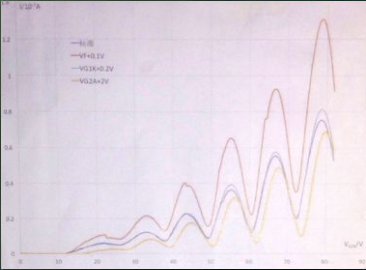
\includegraphics{lab2151_1.png}
    \caption{四条曲线对比图(仅供参考,实际图片请根据实验数据自行绘制)}
	\end{figure}

\subsection*{5.示波器自动测量}

\begin{figure}[H]
	\centering
		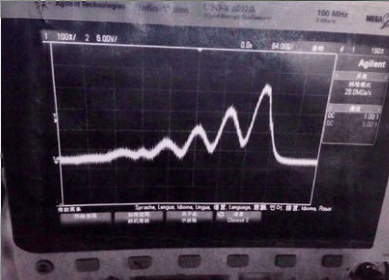
\includegraphics{lab2151_2.png}
	\end{figure}

\end{comment}
\fi
\end{document}